\documentclass[11pt,a4paper]{article}
\usepackage[margin=1in]{geometry}
\usepackage{graphicx}
\title{Q2\_DELIVERY\_2026-03-08\\Scientific Milestone Report}
\author{Science-Chief}
\date{2026-03-08}
\begin{document}
\maketitle

\section*{1. Scope}
This report explains Q2 event-time analysis: cumulative feedback as a function of agent age in block-distance.

\section*{2. Data Provenance and Why We Extracted Them}
On-chain provenance:
Identity Registry \texttt{0x8004A169FB4a3325136EB29fA0ceB6D2e539a432}, Reputation Registry \texttt{0x8004BAa17C55a88189AE136b182e5fdA19dE9b63}.
We extracted these data to measure activation timing after registration and quantify whether feedback arrives quickly or with structural delay.

\section*{3. Extraction and Data Structure}
Core source tables:
\begin{itemize}
\item \texttt{identity\_registered.csv}: registration events with columns such as \texttt{blockNumber, agentId, owner, agentURI}.
\item \texttt{reputation\_newfeedback.csv}: feedback events with columns such as \texttt{blockNumber, agentId, clientAddress, tag1, value, feedbackIndex}.
\end{itemize}
Method:
\begin{enumerate}
\item Match feedback events to registration block by agent ID.
\item Define event-time age: $\Delta b = b_{feedback} - b_{registration}$.
\item Bin by fixed width $\Delta b=1000$ and compute cumulative feedback statistics (mean, median, quartiles).
\end{enumerate}

\section*{4. Results}
\begin{figure}[htbp]
\centering
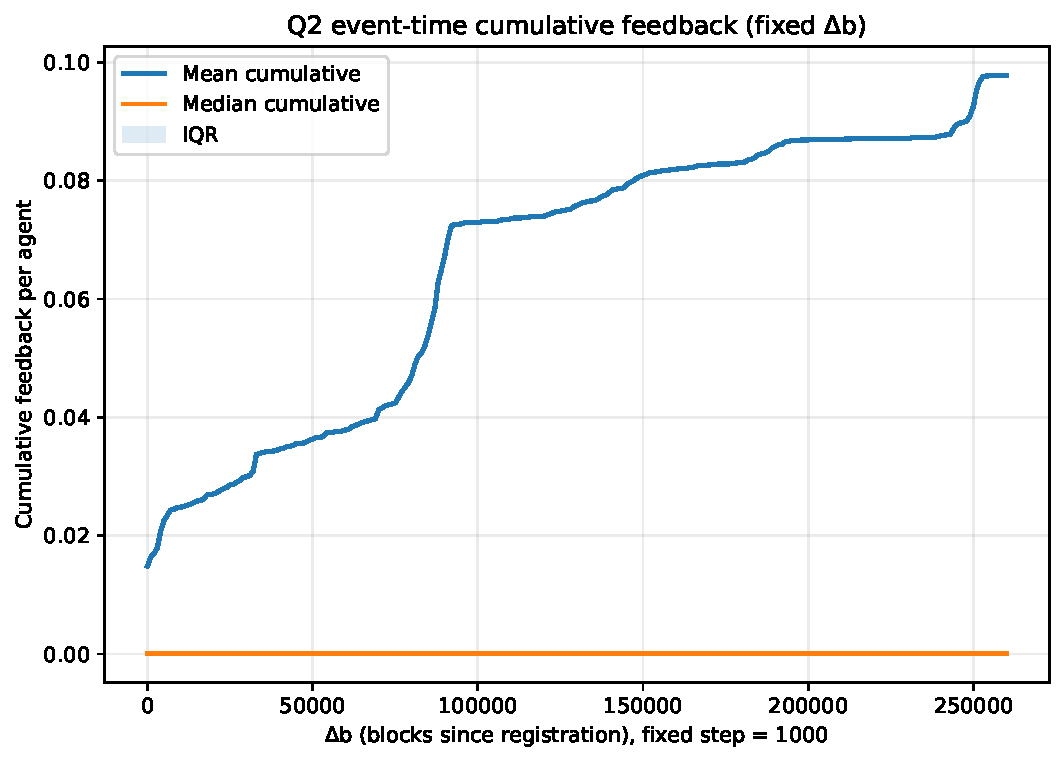
\includegraphics[width=0.9\textwidth]{figures/q2_event_time_cumulative_deltab1000.pdf}
\caption{Cumulative feedback statistics versus event-time.}
\end{figure}
\begin{figure}[htbp]
\centering
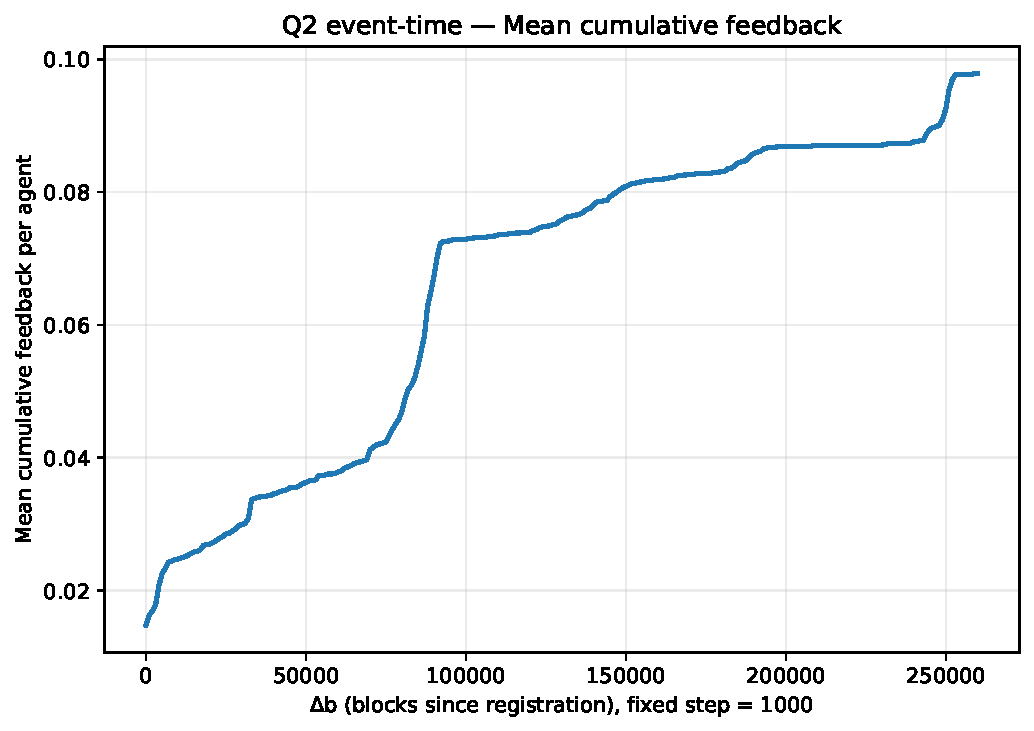
\includegraphics[width=0.85\textwidth]{figures/q2_event_time_mean_deltab1000.pdf}
\caption{Mean cumulative feedback versus event-time.}
\end{figure}
\begin{figure}[htbp]
\centering
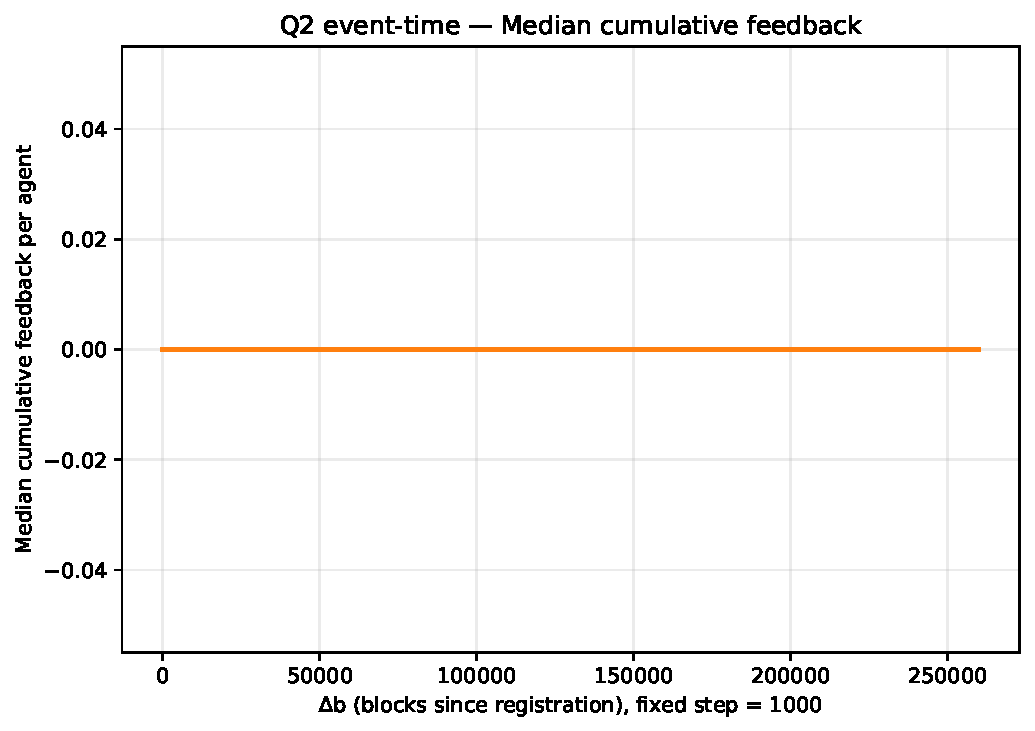
\includegraphics[width=0.85\textwidth]{figures/q2_event_time_median_deltab1000.pdf}
\caption{Median cumulative feedback versus event-time.}
\end{figure}
Key numerical reading: 261 bins up to \texttt{delta\_b=260000}; mean cumulative rises from about 0.0148 to 0.0978, while median remains near zero for most bins.

\section*{5. Scientific Interpretation (SC)}
The event-time panel shows slow and unequal activation: a minority accumulates feedback while the median agent remains inactive for long horizons. This supports the sparse-activation thesis and motivates activated-only robustness checks.

\section*{6. Limitations and Next Steps}
ETH-only scope; block-distance is not calendar time; strong sparsity affects median behavior.
Decision: \textbf{GO internal, HOLD external narrative until robustness extensions are complete}.\
Next: activated-only panel, bin-sensitivity (500/2000), timestamp-enriched variant.

\section*{Appendix: Source Paths}
\textbf{Figures}\\
\begin{itemize}
\item \texttt{workspaces/science-chief/outbox/Reports/Q2\_DELIVERY\_2026-03-08/figures/q2\_event\_time\_cumulative\_deltab1000.pdf}
\item \texttt{workspaces/science-chief/outbox/Reports/Q2\_DELIVERY\_2026-03-08/figures/q2\_event\_time\_mean\_deltab1000.pdf}
\item \texttt{workspaces/science-chief/outbox/Reports/Q2\_DELIVERY\_2026-03-08/figures/q2\_event\_time\_median\_deltab1000.pdf}
\end{itemize}
\textbf{Tables}\\
\begin{itemize}
\item \texttt{workspaces/science-chief/outbox/Reports/Q2\_DELIVERY\_2026-03-08/tables/Q2\_EVENT\_TIME\_CUMULATIVE\_DELTAB1000\_2026-03-08.csv}
\item \texttt{workspaces/science-chief/outbox/Reports/Q2\_DELIVERY\_2026-03-08/tables/q2\_summary\_table.tex}
\item \texttt{workspaces/science-chief/outbox/Reports/Q2\_DELIVERY\_2026-03-08/tables/q2\_checkpoints\_table.tex}
\end{itemize}

\end{document}
